
%%% Local Variables:
%%% mode: latex
%%% TeX-master: t
%%% End:

\chapter{基于 Spark 的分布式近似近邻查询系统}
\label{cha:ANNS_based_on_Spark}
\section{乘积量化}
\label{sec:product_quantization}
与之前提到的 K-Means 的量化方法一样,乘积量化(Product Quantization)\cite{Herve_PQ}也是向量量化方法的一种。假设我们需要量化压缩 128 维的向量到 64 比特,采用 K-Means 的量化方法的话,需要有 $2^{64}$ 个聚类中心,这样不管是从 K-Means 聚类所需要的时间还是从存储聚类中心所占的空间来看,都是不可行的。

对于上面同样的问题,在乘积量化的算法中,我们首先将原始的数据空间划分为 $m$ 个不相交的子空间,也就是将 128 维的向量切成 $m$ 个长度为 $128/m$ 的子向量。在每个子空间里,分别对子空间中的子向量集合进行 K-Means 聚类,聚类中心数量为 $h$。这样我们就可以用 $1\cdots h$ 这些编号来对子向量进行编码,$m$ 个子向量的编码组合在一起就构成了原始向量的编码。这样,原始空间中一个 128 维的向量就可以压缩到一个 $m\log_2h$ 比特编码表示,从而大大节省了空间。
\begin{figure}[H]
  \centering
  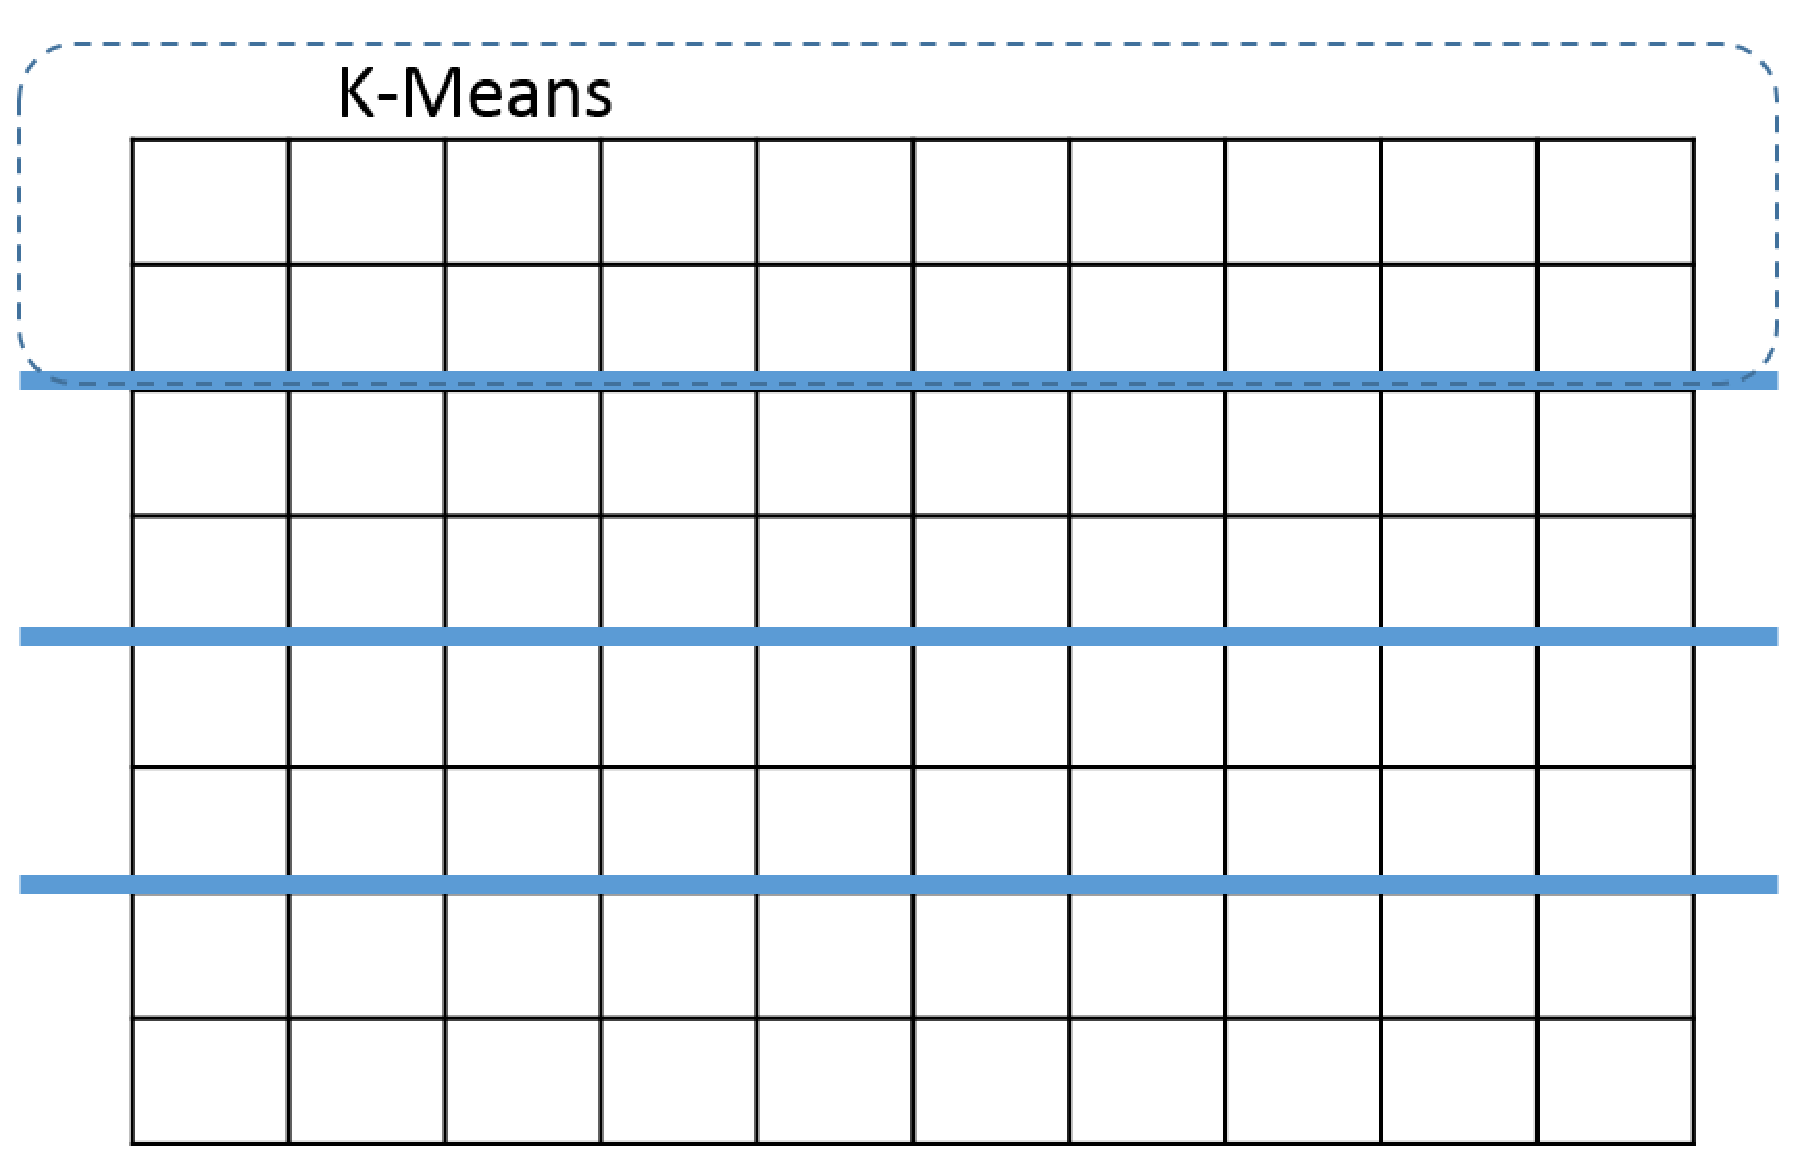
\includegraphics[width=0.5\linewidth]{PQ_subspace}
  \caption{PQ 算法中子空间的划分}
  \label{fig:PQ_subspace}
\end{figure}
更为一般来说,我们可以得到乘积量化方法的目标函数如下:
\begin{equation}
\mathit{l}_\mathrm{PQ} = \sum_{i=1}^n\min\Bigg\lVert \mathbf{x}_i - \begin{bmatrix}C^1\mathbf{b}^1_i\\\vdots\\C^m\mathbf{b}^m_i\end{bmatrix} \Bigg\rVert _2^2
\end{equation}

其中 $\mathbf{x}_i$ 的维度是 $p$,$\mathbf{b}^j_i \in \{0,1\}^h$且$\lVert\mathbf{b}^j_i\rVert=1$,$j \in \{1,\cdots,m\}$。在上面式子中,$C^j(j\in \{1,\cdots,m\})$ 就是我们需要求解的矩阵。在编码过程中,整体的码本(codebook)$C$ 就可以用笛卡尔积的形式表示,$C = C^1 \times \ldots \times C^m$。码本的大小就是所有子空间中聚类中心数量的乘积,根据前面的假设,共有 $m$ 个子空间,每个子空间聚类个数为 $h$,所以码本数量就是 $k = h^m$。求解过程其实并不复杂,正如前文提到,在每个子空间中做 K-Means 聚类就可以求解出码本,这样我们就可以利用码本对每个子空间中的子向量进行编码,从而对原始向量进行编码表示。整个算法的复杂度就和向量维度 $p$、子空间数量 $m$、子空间聚类中心数量 $h$ 有关,存储码本所需要的空间复杂度为 $O(mhp)$。
\begin{table}[htbp]
  \centering
  \caption{乘积量化与 K-Means 量化的空间占用对比}
  \label{tab:kmean_pq}
  \begin{minipage}[t]{0.61\textwidth}
    \begin{tabular}{|c|c|c|c|}
      \hline
                    & 聚类中心 & 编码长度& 空间占用\\
      \hline
      K-Means 量化  &  $k$ &   $\log k$&   $O(kp)$\\
      乘积量化      &   $h^m$ &   $m\log h$ &  $O(mhp)$\\
      \hline
    \end{tabular}\\[2pt]
    \footnotesize 注:$h^m = k$
  \end{minipage}
\end{table}

从表 \ref{tab:kmean_pq} 是乘积量化算法和 K-Means 量化算法的空间占用对可知,当 $m = 1$ 时,乘积量化就退化成普通的 K-Means 聚类量化了。此外, $h$ 取值越大,不仅计算时间复杂度越大,而且空间复杂度也越大,进而也会使得在查询时的时间复杂度变大。因此,选择一个合适的 $m$ 和 $h$ 是非常重要的。论文\cite{Herve_PQ}中指出,$ m = 8 $ 和 $h = 256$ 是比较合适的选择。
\section{基于乘积量化的近似近邻查询}
刚刚我们已经介绍了乘积量化的编码压缩方法,那么如何将这一方法运用在近似近邻查询当中呢?采用乘积量化的方法进行近似近邻查询也是一个机器学习类方法,遵循学习类算法的主体流程。整个近似近邻查询算法的主要流程如下:
\begin{itemize}
\item 利用部分数据集,依照乘积量化的方法训练出码本。
\item 在原始的数据集上,采用训练出的码本对其进行编码压缩。
\item 对于任意的查询向量,度量它与编码压缩后的码字之间的距离,从而得到近邻集合。
\end{itemize}
\subsection{训练码本}
首先是训练集的选择,训练集的选取对整个算法是非常关键的,最终近邻查询的准确率一定程度上取决于训练集的好坏。在选择训练集上有两点需要注意,一是训练集的规模大小,二是训练集的代表性。训练集的规模既不宜过大也不能太小,过大会带来过拟合问题,过小则会欠拟合。通常,训练集的规模大小约为原始数据集的 $1/10$ 比较合适。此外,训练集还应该尽可能得有代表性,尽可能广泛地分布于整个数据空间,这样才能使得训练出来的码本才能更好的量化原始数据空间,更准确地对原始数据集进行编码。

在具体训练码本的过程中,如章节 \ref{sec:product_quantization} 中所介绍的一样,首先将训练集中的数据划分到 $m$ 个子空间。在每个子空间中,对所有的子向量数据在进行 K-Means 聚类,可以得到 $h$ 个聚类中心,也就得到每个子空间的码本。算法的伪代码如算法 \ref{algo:train} 所示。
\begin{algorithm}
    \caption{训练码本}
    \label{algo:train}
    \begin{algorithmic}[1] %每行显示行号
        \Require 训练集 $C$ 矩阵,子空间聚类数量 $subCenters$,聚类算法最大迭代次数 $maxIterations$
        \Ensure 码本模型数组 $model$
        \Function {PQ\_TRAIN}{$C, subCenters, maxIterations$}
            \State uniformly split $C$ by rows into $m$ part
            \For{$i = 1 \to m $}
                \State $model[i] \gets KMEANS\_TRAIN(C[i], subCenters, maxIterations)$
            \EndFor
            \State \Return{$model$}
        \EndFunction
    \end{algorithmic}
\end{algorithm}
\subsection{编码压缩}
如算法 \ref{algo:assgin} 所示,训练得出每个子空间中的码本之后,将其应用到原始数据集上进行编码压缩。首先,同样也是将原始数据集划分到 $m$ 个子空间。然后在每个子空间中,对每一个数据的子向量,分别用训练出来的码本进行编码,也就是用训练好的 K-Means 模型进行预测,可以知道每个子向量隶属于哪个聚类中心,即子向量应该用哪个码字来编码了。这样,整个数据集中的数据都可以用编码来进行表示。完成编码压缩之后,编码后的数据集相比于原始数据集,存储空间成倍的缩小了。
\begin{algorithm}
    \caption{编码压缩}
    \label{algo:assgin}
    \begin{algorithmic}[1] %每行显示行号
        \Require 码本模型数组 $model$,原始数据集 $X$ 矩阵
        \Ensure 编码后的矩阵 $B$
        \Function {PQ\_ASSIGN}{$model, X$}
            \State uniformly split $X$ by rows into $m$ part
            \For{$i = 1 \to m $}
                \For{$j = 1 \to n $}
                    \State $B[i][j] \gets model[i].predict(X[i][j])$
                \EndFor
            \EndFor
            \State \Return{$B$}
        \EndFunction
    \end{algorithmic}
\end{algorithm}
\subsection{近邻查询}
在近似近邻查询的过程中,对于任意一个查询向量 $q$,我们首先计算出 $q$ 在子空间中对应子向量和子空间中聚类中心之间的距离,将计算出的距离用一个查找表存储好。现在我们计算查询向量 $q$ 和编码数据集上的每个数据之间的距离。在每个子空间中,因为我们已经计算出了子向量与聚类中心之间距离,利用查找表,我们就可以迅速得出每个数据在子空间中与向量对应距离。最终将不同子空间中同一向量距离加和。这样就得到了最终的每个向量和查询向量 $q$ 之间的距离。利用一个优先队列,我们就可以快速获取出前 $k$ 个近邻集合。具体算法流程可以参考算法 \ref{algo:ANNS}
\begin{algorithm}
    \caption{近邻近邻查询}
    \label{algo:ANNS}
    \begin{algorithmic}[1] %每行显示行号
        \Require 码本模型数组 $model$,编码数据集 $B$ 矩阵,查询数据 $q$
        \Ensure 近邻集合 $result$ 数组
        \Function {PQ\_SEARCH}{$model, B, q$}
            \For{$i = 1 \to m $}
                \For{$j = 1 \to model[i].subcenters $}
                    \State $d[i][j] \gets COMPUTE\_DIST(model[i].center[j], q) $
                \EndFor
            \EndFor

            \For{$i = 1 \to n $}
                \State $dist[i] \gets 0$
                \For{$j = 1 \to m $}
                    \State $dist[i] \gets dist[i] + d[i][B[j][i]]$
                \EndFor
            \EndFor
            \State $result = GET\_TOPK(dist)$
            \State \Return{$result$}
        \EndFunction
    \end{algorithmic}
\end{algorithm}
\section{基于 Spark 的分布式近似近邻查询}
\subsection{算法流程设计}
算法的总体流程设计图如图 \ref{fig:algorithm-desgin} 所示,首先在训练数据集上进行码本的训练,得到码本模型后将其运用在原始数据集上进行编码压缩,从而可以将原始数据进行编码表示。最终,对于任意一个查询向量,通过近似近邻查询算法在编码数据集上找出近邻候选集合。
\begin{figure}[H]
  \centering
  \includegraphics[width=0.8\linewidth]{algorithm-desgin}
  \caption{算法总体设计图}
  \label{fig:algorithm-desgin}
\end{figure}
\subsection{数据结构}
在 Spark 上,分布式程序的编写必须依赖分布式的数据结构 RDD, RDD 分布式地存储在不同节点上,这样才能保证程序分布式地执行 。因此如何合理设计程序的 RDD 非常重要。

在 Spark MLlib 库中提供了一种自带的数据结构 BlockMatrix。BlockMatrix 是用 RDD 构建的分布式矩阵,其中 RDD 的类型是 ((Int, Int), Matrix)。(Int,Int)是 Matrix 的下标索引,那么 BlockMatrix 的每一个元素都是一个带下标索引矩阵。BlockMatrix 还提供了一些自带的函数可供调用,如 add、multiply。

\begin{figure}[H]
  \centering
  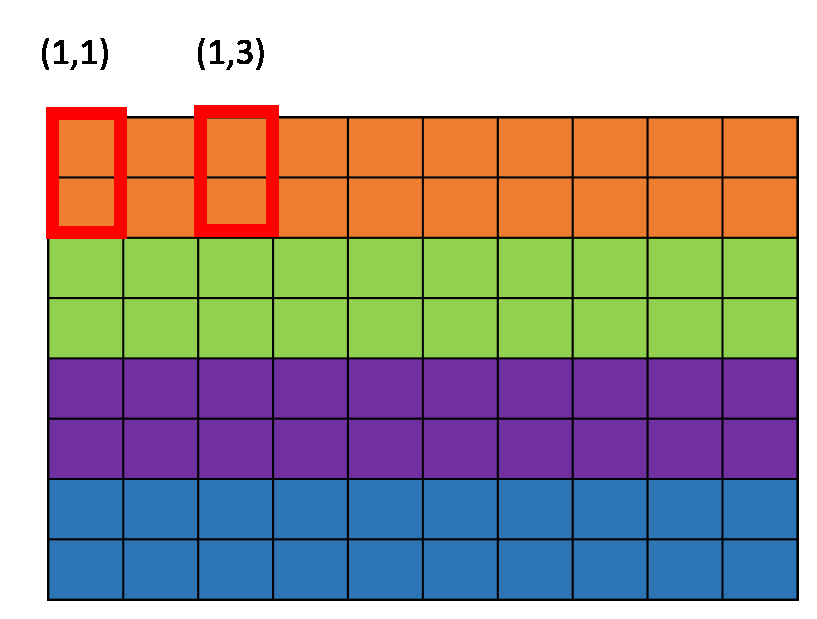
\includegraphics[width=0.6\linewidth]{blockmatrix}
  \caption{BlockMatrix 划分方式}
  \label{fig:blockmatrix}
\end{figure}

图 \ref{fig:blockmatrix} 是一个示例的 BlockMatrix 的划分方式,图中的$ 8\times 10$ 的矩阵被划分成 4 个子空间,每个子空间上有 10 个子向量。那么我们需要一个 $4\times 10$ 的 BlockMatrix 来存储,红色的框中的向量就对应了一个 matrix,相应 matrix 的下标索引标示在图中了。在上一章节的算法中已经说明,我们需要划分 $m$ 个子空间,每个子空间中有 $n$ 个子向量,因此我们用 $m\times n$ 的 BlockMatrix 数据结构来表示数据是比较合适的。具体而言,我们算法中的训练集数据、原始数据、编码后的数据等都是需要用 BlockMatrix 这个数据结构来存储表示的。
\subsection{系统优化}
集群系统上的分布式程序一般来说都会需要考虑通信的问题,即使 Spark 中 RDD 已经进行了很好的封装,让用户可以专注于程序的设计,不用直接进行底层的数据数理(通信、容错)。开发者只需要通过操作上层的一些 API 就可以了,但是数据通信的问题在 Spark 中还是一个不能忽视的问题,只有了解底层的通信机制利用 API 编写出高效的程序。一般来说,我们优化的原则是尽可能地减少数据的通信,特别是通信量比较大的。

数据都是分布式存储,如果某个操作与两个分布式数据同时关联,比如两个大小相同分布式矩阵对应元素相加,那么必须要两个分布式数据中分块的一一对齐。具体到本算法中,根据上一小节所提的数据结构的划分方式,假设存储训练数据集的矩阵用 $C$ 表示,存储原始数据集 BlockMatrix 用 $X$ 表示,存储编码后数据集的矩阵用 $B$ 表示,这些都是分布式地存储在集群系统当中的。由于子空间的划分,我们会在每个子空间中生成自己的码本模型。如果码本模型是分布式存储,那么在编码阶段,我们需要将子空间对齐。 Spark RDD 的 join 操作确实提供了按照键值进行对齐操作,但这一过程可能就会产生一些数据分区重组操作。这种分区重组的操作需要进行磁盘读写和网络,因此我们应该尽量避免 分区重组操作。我们考虑采用 RDD 的广播操作,一次性将只读的数据广播到集群上的所有节点,每个节点上的任务在执行过程中可以直接读取,而不需要考虑对齐问题。在我们算法中,我们选择将计算出的码本模型广播到所有节点以便编码阶段使用。

第二点优化就是利用之前提到的 Spark RDD 的持久化机制。Spark RDD 的持久化可以将 RDD 数据缓存到内存或者磁盘上,以后用到 RDD 的时候不要再次重复计算,从而节省时间效率,这一机制特别适合迭代计算中使用。在我们的算法中,我们选择将一些反复用到 RDD 缓存在内存当中。
\section{本章小结}
本章中首先介绍了乘积量化的哈希方法,通过乘积量化的方法将原始数据集进行编码压缩。之后,我们还介绍了乘积量化哈希方法在近似近邻查询中应用。通过训练码本、编码压缩、近似近邻查询三个过程,我们就可以实现一套完整的近似近邻查询算法。此外,本章节还介绍了在 Spark 计算框架上的这一算法的实现,主要介绍了算法总体流程设计、数据结构的选择以及系统的优化方法。


